% The introduction has to say that transformers have a tape where they recibe the input and write its output

In this work we are going to analyze transformers as language recognizers.
A transformer is a machine that works over an alphabet $\Sigma$.
It has a single tape from which it reads the input and onto which it appends additional tokens in an autoregressive manner.
There are two distinguished tokens called \textbf{decision symbols}.
Once the transformer writes one of those, it halts.
We say that a transformer accepts a word if, when it halts, the decision symbol printed is the accepting one ($\qaccept$).
Analogously, a transformer rejects a word if the decision symbol printed is the rejecting one ($\qreject$).

In each step, the transformer maps the content of the tape to a probability distribution over $\Sigma$.
Then, depending on this distribution, the transformer prints the next token.
The transformer iterates this process until it halts.
These iterations are called \textbf{chain of thought}. \rafa{Agregar una cita}

We split the process of generating the next token into two separate steps.
First, the computation of the probability distribution over the alphabet which we call distribution generation.\bigsanti{así como hiciste con cot, definí nuevos términos con un estilo especial. Yo uso defstlye como comando y después decido si es itálica, negrita, etc} \bigrafa{defino distribution generation y token selection más abajo y los puse en negrita. Debería marcarlos también acá?}
Second, the selection of a token based on the probability distribution, which we call token selection.
In this work we analyze and compare two different algorithms for token selection.

\medskip

Most prior work only considers transformers that operate over an infinite tape.
This is far from the real models, thus the transformers studied in this thesis work over a finite tape.
The size of the tape is defined, for each input size $n$, as $\budget(n) + n$.
It is important to remark that the size of the tape bounds the number of steps of $\CoT$ that the transformer makes.
For an input word of length $n$, no computation can take more than $\budget(n)$ steps because every step writes a token in the tape.


\medskip

The process of distribution generation is dependent on many parameters.
In the real models, these parameters are the ones calculated during the training.


We refer to them as $\theta$ and consider them as part of the definition of a transformer.


\bigskip
%%%%%%%%%%%%%%%%%%%%%%%%%%%%%%%%%%%%%%%%%%%%%%%%%%%%%%%%%%%%%%%
        % Formal general def of transformer and CoT %
%%%%%%%%%%%%%%%%%%%%%%%%%%%%%%%%%%%%%%%%%%%%%%%%%%%%%%%%%%%%%%%

We denote by $\TF(\alpha)$ the token outputted after one step of the computation of the transformer $\TF$ when the tape content is $\alpha \in \Sigma^*$.
The autoregressive token generation is defined recursively.
The token outputted after $i$ steps is $\TF^{i}(\alpha) := \TF^{i-1}(\alpha \TF(\alpha))$ with base case $\TF^1(\alpha) := \TF(\alpha)$.
In other words, the output of the $i$th step is $\sigma_{i} = \TF^{i}(\alpha) = \TF(\alpha\sigma_{1}\dots\sigma_{i-1})$ where $\sigma_j \in \Sigma$ for all $j$.

We denote by $\TF^*(\alpha)$ the token written by the transformer when it halts, i.e., at the end of the computation, when the input is $\alpha$.
As said before, the transformer only halts when it prints a decision symbol ($\qaccept$ or $\qreject$).
Therefore, $\TF^*(\alpha) \in \{\qaccept, \qreject\}$.




\medskip
%%%%%%%%%%%%%%%%%%%%%%%%%%%%%%%%%%%%%%%%%%%%%%%%%%%%%%%%%%%%%%%
            % Def of distribution generator %
%%%%%%%%%%%%%%%%%%%%%%%%%%%%%%%%%%%%%%%%%%%%%%%%%%%%%%%%%%%%%%%


As stated before, the \textbf{distribution generation} is a mapping of the content of the tape to a probability distribution over $\Sigma$.
There are different algorithms for this process in the literature.
All transformers considered in this work employ the one presented in \cite{toyota}.
This algorithm consists of four parts: a token embedding layer ($\TE$), a position encoding layer ($\PE$), an output linear layer ($\OUTPUT$) and a stack of $L$ identical decoder layers, where $L$ is also called the depth of the model. 
Each decoder layer has two sub-layers: a multi-head self-attention layer ($\ATTN$) and a position-wise fully-connected feed-forward network ($\FF$). 
Each part and layer has its own trainable parameters.
Then, we can define the distribution generation algorithm by its parameters $\theta = \{\theta_\TE, \theta_\PE, \{\theta_\ATTN^{l}, \theta_\FF^{l}\}_{l=0}^{L-1}, \theta_\OUTPUT\}$.
The algorithm works over vectors of numbers of certain dimension $d$.
The dimension is dependent on the size of the input word.
We call $d(n)$ to the \textbf{embedding size} when the input word has size $n$.

%Each part
\textbf{Token Embedding:} It is a mapping from $\Sigma$ to vectors in $\Rd$. 
This mapping is defined by $\theta_{\TE} \in \mathbb{R}^{d \times | \Sigma |}$. 
For all $\sigma \in \Sigma$, we note $\theta_{\TE}(\sigma) \in \mathbb{R}^d$ to the mapping of token $\sigma$.

\textbf{Position Encoding:} It is a mapping from the positions of the tape to vectors in $\Rd$.
This mapping is defined by $\theta_{\PE} \in \mathbb{R}^{d \times \budget(n) + n}$. 
For all position of the tape $1 \leq i \leq \budget(n) + n$ we note $\theta_{\PE}(i) \in \Rd$ to the mapping of position $i$.

\bigcifu{Intuición de todas estas capas?}
\bigrafa{Lo hago en la intro? Me parece el mejor lugar para hacerlo}

\textbf{Self Attention Layer: } It is a mapping from $(\Rd)^a$ to $(\Rd)^a$.
Given parameters $\theta_{\ATTN} = (W_Q, W_K , W_V , W_O) \in \mathbb{R}^{d \times d} \times \mathbb{R}^{d \times d} \times \mathbb{R}^{d \times d} \times \mathbb{R}^{d \times d}$, the layer is defined by the algorithm \ref{alg:def_attn}. 
This layer is defined only as a single head attention layer because a multi-head attention layer with any constant number of heads can be simulated with multiple single-head attention layers \cite{cookbook}.

\begin{algorithm}
\caption{Causal Self-Attention, $\ATTN$}\label{alg:def_attn}
\begin{algorithmic}[1]
\Input Parameter $\theta_\ATTN = (W_Q,W_K,W_V,W_O)$ and embedding $h= (h_1,\ldots, h_a)\in\Rd \times \dots \times \Rd$.
\Output Embedding $h'= (h'_1,\ldots, h'_a) := \ATTN_{\theta_\ATTN}(h_1,\ldots, h_a)$.
\State $q_i := W_Q  h_i, \; k_i := W_K h_i, \; v_i := W_V h_i, \; \forall i\in[1, \dots, a]$
\State $s_i := \softmax (\langle q_i, k_1 \rangle, \ldots, \langle q_i, k_i\rangle) \| (0,\ldots, 0) $
\State $h'_i := W_O \sum_{j=1}^a (s_i)_j v_j$
\end{algorithmic}
\end{algorithm}

\textbf{Feed Forward Network: } It is a mapping from $\Rd$ to $\Rd$. Given $\theta_{\FF} = (W_1 , b_1 , W_2 , b_2) \in \mathbb{R}^{d \times d} \times \Rd \times \mathbb{R}^{d \times d} \times \Rd$, the layer is defined as $\FF_{\theta_\FF}(h) := W_2 \; \relu(W_1 h + b_1 ) + b_2$, where $\relu: \mathbb{R}^d \to \mathbb{R}^d$ replaces each position $x_i$ by $\text{max}(0, x_i)$.


\textbf{Output Layer: } It is a mapping from $\Rd$ to a probability distribution over $\Sigma$.
Given $\theta_{\OUTPUT} \in \mathbb{R}^{| \Sigma | \times d}$, we define it as $\OUTPUT_{\theta_\OUTPUT}(h) := \softmax(\theta_\OUTPUT h)$.


All these parts come together for the distribution generator process in the algorithm \ref{alg:def_p_gen}.

\begin{algorithm}
\caption{Distribution generator}\label{alg:def_p_gen}
\begin{algorithmic}[1]
\Input Transformer parameter $\theta = (\theta_\TE, \theta_\PE, \{\theta_\ATTN^{l}, \theta_\FF^{l}\}_{l=0}^{L-1}, \theta_\OUTPUT)$ and tokens of the tape $\alpha \in \Sigma^*$.
\Output distribution $p_\theta(\cdot | \alpha)$.
\State $h^{(0)}_i \gets \theta_\TE(\alpha_i) + \theta_\PE(i), \; \forall 1 \leq i \leq |\alpha|$
\For{$l = 0,\ldots,L-1$}
\State	$( h^{(l+0.5)}_1,\ldots, h^{(l+0.5)}_{|\alpha|}) \gets (h^{(l)}_1,\ldots, h^{(l)}_{|\alpha|}) +\ATTN_{\theta^{(l)}_\ATTN}(h^{(l)}_1,\ldots, h^{(l)}_{|\alpha|}) $
\State  $ h^{(l+1)}_i \gets  h^{(l+0.5)}_i + \FF_{\theta^{(l)}_\FF}(h^{(l+0.5)}_i)$, $\forall 1 \leq i \leq |\alpha|$
\EndFor
\State $p_\theta(\cdot| \alpha) \gets  \OUTPUT_{\theta_\OUTPUT}(h^{(L)}_{|\alpha|})$
\end{algorithmic}
\end{algorithm}

The $\OUTPUT$ layer and the $\ATTN$ layer use a $\softmax$ function $\mathbb{R}^n$ to $\mathbb{R}^n$ defined as $\softmax(x)_i = exp(x_i) / \sum_{j=1}^n exp(x_j)$.

\medskip

%%%%%%%%%%%%%%%%%%%%%%%%%%%%%%%%%%%%%%%%%%%%%%%%%%%%%%%%%%%%%%%%%
                % Def token selection %
%%%%%%%%%%%%%%%%%%%%%%%%%%%%%%%%%%%%%%%%%%%%%%%%%%%%%%%%%%%%%%%%%

The second component of a transformer is the \textbf{token selector}.
This algorithm consumes the probability distribution computed by the distribution generator and returns a token.

In this work we study two selectors, we call them \textbf{deterministic selector} and \textbf{probabilistic selector}.
Let $p \in \Delta(\Sigma)$ be the distribution over $\Sigma$ outputted by the distribution generator.
Then, the deterministic selector always returns the token with the largest probability ($\argmax$ over $p$).
In transformers with this selector, we do not allow for two or more tokens to be tied with the maximum probability, i.e., $\nexists \sigma$ s.t. $p(\argmax(p)) = p(\sigma) \land \sigma \neq \argmax(p)$.
In contrast, the probabilistic selector works non-deterministically.
It returns a token $\sigma \in \Sigma$ with probability $p(\sigma)$.
We allow for more than one maximum with this selector.

\begin{figure*}
    \centering
    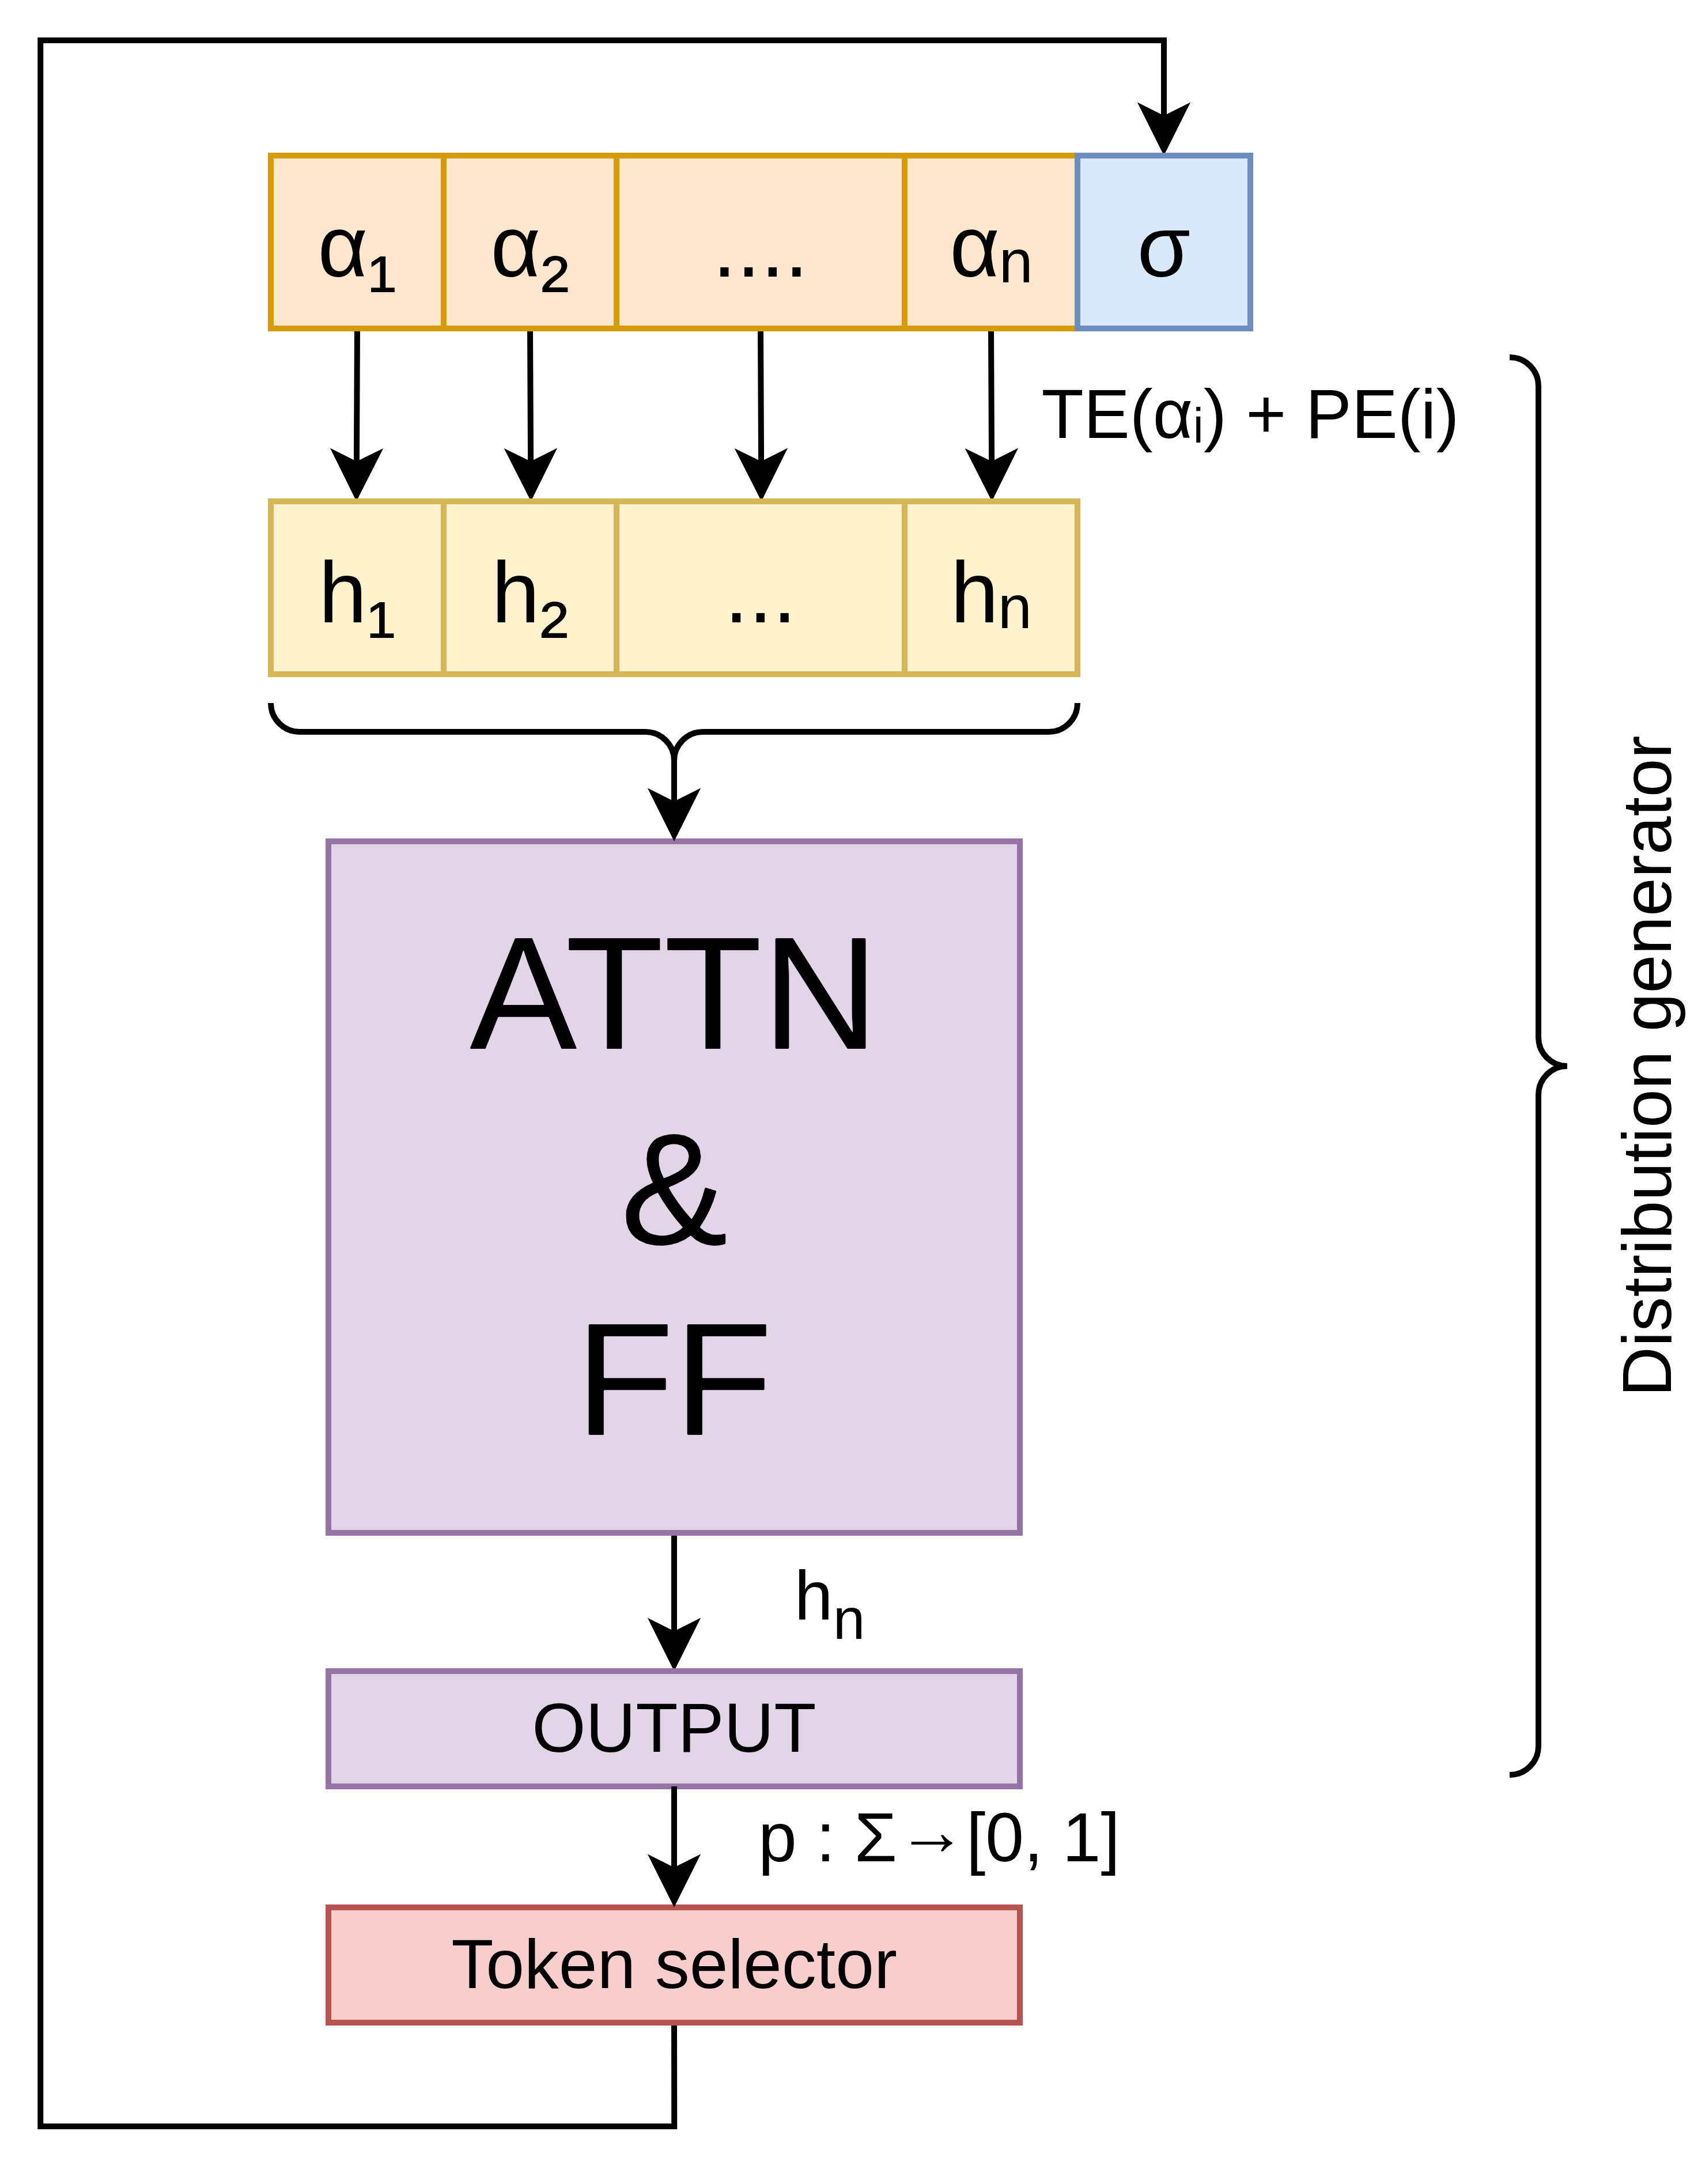
\includegraphics[width=0.5\textwidth]{chapters/diagrams/diagram-transf.png}
    \caption{Transformer architecture}
\end{figure*}




Although the presentation for transformers introduced in this section operates over real numbers, the transformers analyzed during this work utilize $\Floating$ for representing them.
The formal construction is the same, but all operations over the set of real numbers are replaced but their corresponding in the set of $\Floating$ numbers.
\bigrafa{Toyota tiene copiado lo mismo que está en esta sección en un apéndice donde hizo ctrl +f y reemplazo $\mathbb{R}$ por $\Floating$. Vale la pena que haga lo mismo?}